\chapter{Les plugins indispensables}

Soyons clair, \vim sans ses plugins, c'est comme Milan sans Rémo\sidenote{\copyright François Corbier - Sans ma barbe - \url{http://www.bide-et-musique.com/song/149.html}} : ça ne rime à rien. C'est grâce aux plugins que \vim va pouvoir pleinement exprimer toute sa puissance et vous élever à un autre niveau de productivité. Vous n'avez pas besoin d'en avoir des mille et des cents, mais quelques uns savamment choisis devraient faire l'affaire.

Qu'on ne se méprenne pas, \vim peut bien sûr s'utiliser sans plugins. Il peut d'ailleurs s'avérer utile de savoir faire les manipulations de base sans avoir besoin d'installer de plugin, car c'est souvent le cas sur des serveurs : il n'y a aucun plugin d'installé. Dans ce cas là, savoir ouvrir, sauvegarder sous, passer d'un fichier à l'autre avec les commandes de \vim par défaut peut vous sauver la mise. En revanche, dans votre travail quotidien de rédaction ou de code, les plugins sont indispensables pour pleinement tirer partie de \vim.

\section{Naviguer sur le disque et entre les fichiers : \emph{Lusty Explorer}}

Nous avons déjà vu NerdTree dans \nameref{ssec:nerdtree} qui permettait d'avoir un explorateur de projet dans une fenêtre latérale de \vim. Le problème de ce plugin est qu'il n'est pas fait pour être utilisé au clavier. Certes vous pouvez utiliser le clavier, mais il ne sera pas aussi efficace que les plugins pensés uniquement pour une utilisation au clavier.

Personnellement, le premier plugin que j'installe partout où j'ai à utiliser \vim, c'est \emph{Lusty Explorer}\sidenote{\url{http://www.vim.org/scripts/script.php?script\_id=1890}}. Ce plugin va vous permettre de naviguer sur votre disque dur pour ouvrir facilement des fichiers en se passant de la souris. Il va aussi permettre de naviguer rapidement entre vos différents fichiers déjà ouverts (vos buffers on jargon \vim). Commençons par l'installer.

Rendez-vous sur l'url du script \url{http://www.vim.org/scripts/script.php?script\_id=1890} et télécharger la dernière version (c'est actuellement la 4.3)\sidenote{\url{http://www.vim.org/scripts/download\_script.php?src\_id=17529}}. Faites ensuite le nécessaire dans votre répertoire \Verb|.vim/| pour qu'il ressemble à la structure ci-dessous :

\begin{verbatim}
.vim
|-- autoload
|   `-- pathogen.vim
`-- bundle
    |-- lusty-explorer
    |   `-- plugin
    |       `-- lusty-explorer.vim
\end{verbatim}

Si vous avez suivi tout ce que l'on a fait depuis le début votre répertoire \dotvim, il devrait maintenant ressembler à cela :

\begin{verbatim}
.vim
|-- autoload
|   `-- pathogen.vim
`-- bundle
    |-- lusty-explorer
    |   `-- plugin
    |       `-- lusty-explorer.vim
    |-- nerdtree
    |   |-- doc
    |   |   `-- NERD_tree.txt
    |   |-- nerdtree_plugin
    |   |   |-- exec_menuitem.vim
    |   |   `-- fs_menu.vim
    |   |-- plugin
    |   |   `-- NERD_tree.vim
    |   `-- syntax
    |       `-- nerdtree.vim
    `-- solarized
        `-- colors
            `-- solarized.vim
\end{verbatim}

Reste à voir comment l'utiliser. Si l'on se réfère à la documentation, voilà ce que l'on trouve (traduit en français) :

\begin{verbatim}
<Leader>lf  - Ouvre l'explorateur de fichiers.
<Leader>lr  - Ouvre l'explorateur de fichiers à partir du répertoire du fichier courant.
<Leader>lb  - Ouvre l'explorateur de buffers.
<Leader>lg  - Ouvre la recherche dans les buffers.
\end{verbatim}

On voit qu'il est fait mention d'une touche nommée \tleader qu'il faut ensuite faire suivre d'autres touches comme \emph{lf}, \emph{lr}, \emph{lb} et \emph{lg}. Cette touche \tleader\xspace est une touche spéciale que l'on définit dans son fichier \vimrc. Elle sera énormément utilisée par tous les plugins, beaucoup des commandes de ces derniers commenceront par la touche \tleader. C'est un moyen d'éviter les collisions avec les raccourcis par défaut de \vim.

Il faut donc choisir une touche \tleader. Par défaut, \vim utilise \textbackslash\xspace comme touche \tleader. Sur nos claviers francophones c'est une très mauvaise idée d'utiliser cette touche car elle n'est pas pratique du tout. La plupart des utilisateurs de \vim la remplace par la touche \tcomma. Elle est directement accessible sous l'index de la main droite ce qui en fait une parfaite candidate. Pour spécifier cela à \vim il va falloir rajouter une ligne dans votre fichier \vimrc, à savoir :

\begin{listing}[H]

    \begin{minted}[bgcolor=bg, gobble=8]{vim}
        let mapleader = ","
    \end{minted}
    \caption{Spécifier la touche leader.}
    \label{code:leader}
\end{listing}

Une fois la modification effectuée et prise en compte (en redémarrant \vim ou en tapant \vimcmd{:source \~{}/.vimrc} en mode normal), vous devriez être en mesure de taper \vimshortcut{,lr} et d'avoir le même style de résultat que sur la figure \ref{fig:vim-lusty}.

\begin{figure}%
  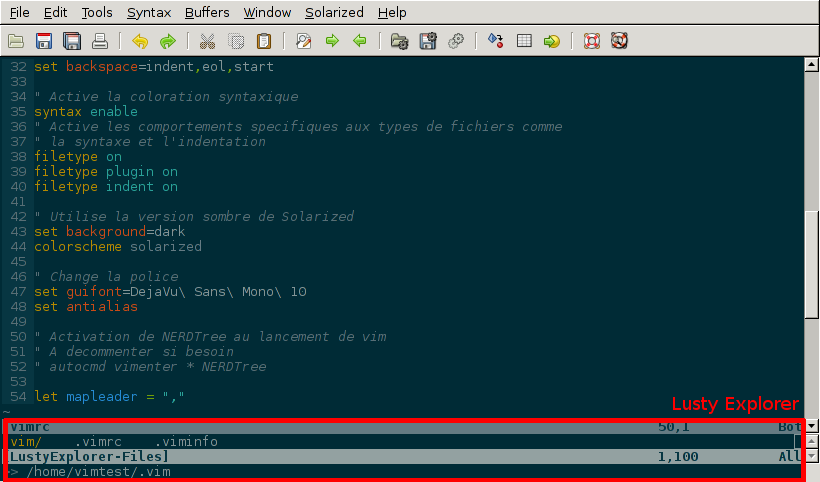
\includegraphics[width=\linewidth]{vim-lusty.png}
  \caption{\vim avec Lusty Explorer d'activé en bas.}
  \label{fig:vim-lusty}
\end{figure}

Je vous conseille maintenant de désactiver \emph{The Nerd Tree} (en commentant la ligne au dessus du \emph{mapleader} comme je l'ai fait dans la figure \ref{fig:vim-lusty-fuzzy}), il ne vous servira plus à grand chose, \emph{Lusty Explorer} le remplace à merveille.

Vous pouvez constater sur la figure \ref{fig:vim-lusty} qu'il y a deux parties à \emph{Lusty Explorer}. La partie basse vous indique le répertoire que vous êtes en train d'explorer et la partie haute liste le contenu de ce répertoire. En surbrillance se trouve l'élément couramment sélectionné. Dans le cas de la figure \ref{fig:vim-lusty} c'est le répertoire \Verb|.vim/| en jaune  (la couleur pourra être différente en fonction de votre thème).

\emph{Lusty Explorer} utilise une fonctionnalité de \emph{Fuzzy matching} qui va vous permettre de ne taper qu'une partie d'un nom de fichier pour le sélectionner. Dans mon exemple, si, dans la fenêtre de \emph{Lusty}, je saisi \Verb|.vimi| il va me sélectionner le fichier \Verb|.viminfo| sans que j'ai à lui spécifier le nom entier, je n'aurais ensuite plus qu'à appuyer sur \ttenter pour ouvrir le fichier dans \vim. La figure \ref{fig:vim-lusty-fuzzy} vous montre l'exemple en question.

\begin{figure}%
  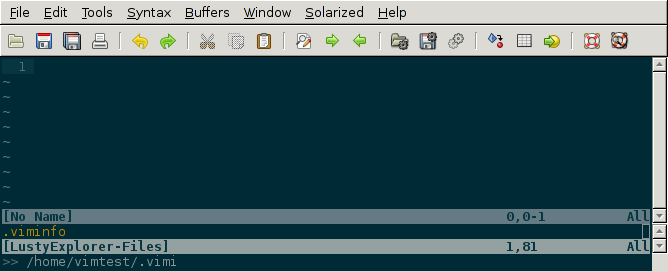
\includegraphics[width=\linewidth]{vim-lusty-fuzzy.png}
  \caption{Lusty Explorer et le Fuzzy matching.}
  \label{fig:vim-lusty-fuzzy}
\end{figure}

\emph{Lusty Explorer} dispose en plus de quelques raccourcis bien pratiques pour utiliser le navigateur de fichiers :

\begin{itemize}
    \item \tctrl + \tn\xspace pour sélectionner le fichier/répertoire suivant
    \item \tctrl + \tp pour sélectionner le fichier/répertoire précédent
    \item \tctrl + \tw pour descendre au répertoire parent
    \item \tctrl + \te crée un nouveau fichier vide (non sauvegardé sur le disque) avec le nom spécifié actuellement dans \emph{Lusty Explorer}. Vous n'aurez plus qu'à utiliser \vimcmd{:w} pour écrire le contenu du fichier sur le disque.
\end{itemize}

\emph{Lusty Explorer} s'utilise donc pour deux choses : naviguer sur votre système de fichiers avec \vimshortcut{,lr} et \vimshortcut{,lf}, et naviguer entre vos fichiers ouverts (buffers) avec \vimshortcut{'lb}. Personnellement j'utilise moins la recherche dans les buffers avec \vimshortcut{,lg}, à vous de tester et de vous faire votre propre opinion.

Je vous conseille en guise de test d'ouvrir plusieurs fichiers avec \vimshortcut{,lr} ou \vimshortcut{,lf}. Ensuite, entraînez-vous à naviguer entre ces différents fichiers ouverts en même temps à l'aide de \vimshortcut{,lb}. C'est une des combinaisons que j'utilise le plus au quotidien.

Ce plugin est indispensable et ajoute à lui seul énormément de valeur à \vim : se passer de la souris pour ouvrir des fichiers. Prenez donc le temps nécessaire pour l'apprendre correctement, c'est un investissement qui vaut le coup.

\section{Recherche dans les fichiers sur le disque : \emph{Ack}}

Lorsque l'on édite un fichier appartenant à un projet plus gros contenant lui même beaucoup de fichiers, il arrive souvent de vouloir rechercher une occurrence d'une chaîne de caractères dans tous les fichiers du projet. Pour ce faire, \vim dispose d'un plugin permettant d'utiliser \emph{Ack} pour faire cette recherche.

\emph{Ack}\sidenote{\url{http://betterthangrep.com/}} est un programme écrit en \emph{perl} qui remplace avantageusement le bon vieux \emph{grep} pour effectuer des recherches dans des fichiers. Il a en revanche un désavantage par rapport à \emph{grep} : il est rarement installé par défaut. Nous allons donc commencer par installer \emph{Ack} avant de pouvoir aller plus loin. Cela va bien sûr dépendre de la plateforme sur laquelle vous utilisez \vim, vous pourrez trouver différentes instructions en fonction de votre plateforme sur la page du plugin : \url{http://github.com/mileszs/ack.vim#installation}.

Pour Debian/Ubuntu : \textbf{\emph{sudo apt-get install ack-grep}}. Pour Mac Os X vous allez avoir besoin de Homebrew (\url{http://mxcl.github.com/homebrew/}) en utilisant \textbf{\emph{brew install ack}}. Pour les utilisateurs de MacPorts ça sera avec la commande \textbf{\emph{sudo port install p5-app-ack}}. Pour Windows installez Strawberry Perl (\url{http://strawberryperl.com/}) et dans le shell de commandes exécutez \textbf{\emph{C:\textbackslash>cpan App::Ack}}. Vous devriez ensuite pouvoir utiliser la commande \textbf{ack} dans votre terminal de commandes en lieu et place de \textbf{grep}.

Rendez-vous sur la page du plugin ack\sidenote{\url{http://www.vim.org/scripts/script.php?script\_id=2572}} et téléchargez la dernière version (à l'heure où j'écris ces lignes c'est la version 0.3.1). Décompressez l'archive dan votre répertoire \Verb|~/.vim/bundle/|, de manière à obtenir une structure de ce type :

\begin{verbatim}

bundle
|-- ack
|   |-- doc
|   |   `-- ack.txt
|   `-- plugin
|       `-- ack.vim
…
\end{verbatim}

Comme d'habitude assurez-vous que vos modifications sont bien prises en compte en redémarrant \vim ou en tapant \vimcmd{:source \~{}/.vimrc} en mode normal.

Il va ensuite falloir ajouter quelques lignes à notre fichier \vimrc pour faciliter d'utilisation du plugin :

\begin{listing}[H]

    \begin{minted}[bgcolor=bg, gobble=8]{vim}
        " Parametres par defaut pour ack
        let g:ackprg="ack -H --nocolor --nogroup --column"
        " Place un marqueur et cherche
        nmap <leader>j mA:Ack<space>
        " Place un marqueur et cherche le mot sous le curseur
        nmap <leader>ja mA:Ack "<C-r>=expand("<cword>")<cr>"
        nmap <leader>jA mA:Ack "<C-r>=expand("<cWORD>")<cr>"
    \end{minted}
    \caption{Configuration du plugin Ack.}
    \label{code:ack}
\end{listing}

Ack recherchera alors à partir du répertoire où se trouve votre fichier couramment ouvert. Vous pouvez faire quelques tests si vous le souhaitez (en supposant que votre touche <leader> est la touche \tcomma :

\begin{itemize}
    \item \vimcmd{,j} \emph{toto} : recherchera \emph{toto} à partir du répertoire du fichier courant,
    \item \vimcmd{,ja} avec votre curseur sur un mot recherchera ce mot.
\end{itemize}

\bigskip

Le plugin Ack vous affichera les résultats dans une fenêtre que l'on appelle \emph{Quickfix Window}, cf image \ref{fig:vim-ack-quickfix}.

\begin{figure}%
  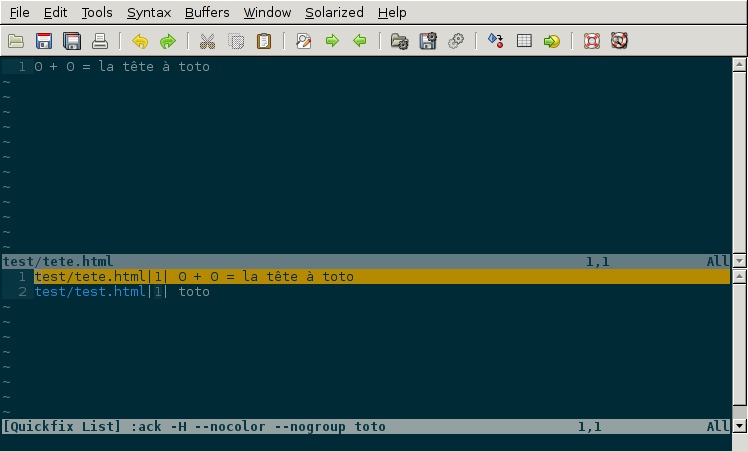
\includegraphics[width=\linewidth]{vim-ack-quickfix.png}
  \caption{\vim avec la fenêtre Quickfix de Ack.}
  \label{fig:vim-ack-quickfix}
\end{figure}


Voici quelques commandes disponibles dans cette fenêtre :

\begin{itemize}
    \item \textbf{o} : ouvrir (idem que <Entrée>
    \item \textbf{go} : voir un aperçu (ouvre le fichier mais mantient le focus sur les résultats de ack.vim)
    \item \textbf{t} : ouvrir dans un nouvel onglet
    \item \textbf{T} : ouvrir dans un nouvel onglet en arrière plan
    \item \textbf{h} : ouvrir en séparant la fenêtre horizontalement
    \item \textbf{v} : ouvrir en séparant la fenêtre verticalement
    \item \textbf{q} : fermer la fenêtre quickfix
\end{itemize}

\bigskip

À noter que par défaut Ack ne recherche que dans les fichiers qu'il reconnait comme pertinents (il ne fera pas de recherche dans les fichiers temporaires, les fichiers des gestionnaires de version, etc.). Si vous souhaitez que Ack recherche dans tous les fichiers indépendamment de leur type, vous devez spécifier l'option \Verb|-u| comme ceci dans votre \vimrc :

\begin{listing}[H]

    \begin{minted}[bgcolor=bg, gobble=8]{vim}
        " Parametres par defaut pour ack
        let g:ackprg="ack -H -u --nocolor --nogroup --column"
    \end{minted}
    \caption{Configuration du plugin Ack pour rechercher dans tous les fichiers.}
    \label{code:leader}
\end{listing}

\section{Recherche de fichiers sur le disque}

Non ce n'est pas pareil que Ack, relisez bien le titre. Ici nous n'allons pas chercher dans les fichiers, mais nous allons plutôt chercher des fichiers à ouvrir avec \vim. Ça peut s'avérer très utile lorsque vous avez travaillez sur des projets où les fichiers sont éparpillés dans un grand nombre de répertoires.

Comme d'habitude nous allons commencer par installer le plugin. Une fois n'est pas coutume, le plugin dispose d'une page dédiée plutôt bien réalisée que vous trouverez ici : \url{http://kien.github.com/ctrlp.vim/}. Scrollez tout en bas pour télécharger la dernière version en "Direct Downloads". Pour les paresseux, voici un lien direct : \url{http://github.com/kien/ctrlp.vim/zipball/master}. Décompressez l'archive dan votre répertoire \Verb|~/.vim/bundle/|, de manière à obtenir une structure de ce type :

\begin{verbatim}

bundle
|
…
|-- ctrlp
|   |-- autoload
|   |   |-- ctrlp
|   |   |   |-- bookmarkdir.vim
|   |   |   |-- buffertag.vim
|   |   |   |-- changes.vim
|   |   |   |-- dir.vim
|   |   |   |-- line.vim
|   |   |   |-- mixed.vim
|   |   |   |-- mrufiles.vim
|   |   |   |-- quickfix.vim
|   |   |   |-- rtscript.vim
|   |   |   |-- tag.vim
|   |   |   |-- undo.vim
|   |   |   `-- utils.vim
|   |   `-- ctrlp.vim
|   |-- doc
|   |   `-- ctrlp.txt
|   |-- plugin
|   |   `-- ctrlp.vim
|   `-- readme.md
…
\end{verbatim}

Comme d'habitude assurez-vous que vos modifications sont bien prises en compte en redémarrant \vim ou en tapant \vimcmd{:source \~{}/.vimrc} en mode normal.

Nous n'avons plus qu'à ajouter un raccourci dans notre \vimrc pour invoquer CtrlP. Dans mon cas j'ai choisi \vimcmd{,c}, mais vous pouvez choisir ce que vous voulez.

\begin{listing}[H]

    \begin{minted}[bgcolor=bg, gobble=8]{vim}
        let g:ctrlp_map = '<leader>c'
    \end{minted}
    \caption{Configuration du raccourci pour activer CtrlP.}
    \label{code:leader}
\end{listing}

La figure \ref{fig:vim-ctrlp} vous montre CtrlP en action.

\begin{figure}%
  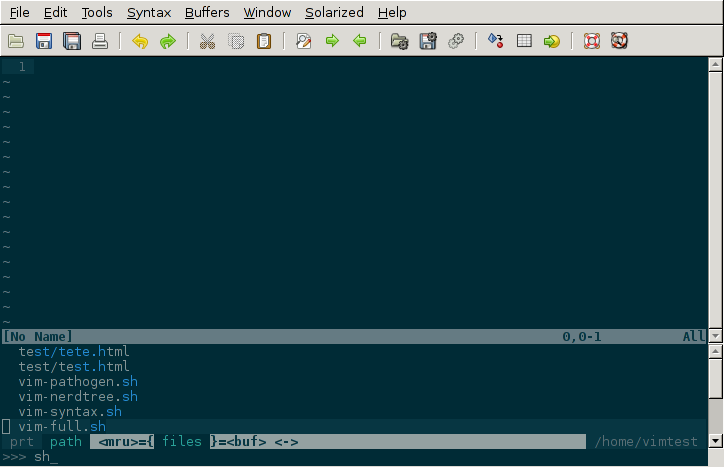
\includegraphics[width=\linewidth]{vim-ctrlp.png}
  \caption{\vim avec CtrlP de lancé.}
  \label{fig:vim-ctrlp}
\end{figure}

À noter que CtrlP peut aussi être utilisé pour naviguer entre les fichiers ouverts (comme Lusty). Mais à l'usage, je le trouve moins pratique que Lusty. Vous pouvez aussi vous en servir pour naviguer automatiquement dans votre code en "suivant" vos fonctions grâce aux tags (comme on peut le faire dans Eclipse). C'est un trop vaste sujet pour être traité dans ce guide, mais si ça vous intéresse vous pouvez déjà consulter cet article de blog sur le sujet : \url{http://andrew-stewart.ca/2012/10/31/vim-ctags} (en anglais).

\section{Les plugins avancés}

neocomplcache : \url{http://www.vim.org/scripts/script.php?script\_id=2620}

surround : \url{http://www.vim.org/scripts/script.php?script\_id=1697}

fugitive : git management \url{https://github.com/tpope/vim-fugitive}

syntastic : checking code syntax \url{https://github.com/scrooloose/syntastic}

ctags + ctrlp : code navigation \url{http://andrew-stewart.ca/2012/10/31/vim-ctags}
